\subsubsection{Boundry-klasse: XboxController}

\begin{figure}[h]
\centering
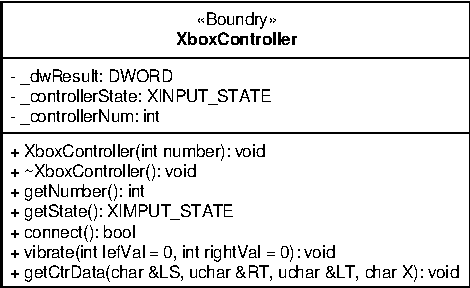
\includegraphics[]{../fig/diagrammer/pc/cd_xboxcontroller.pdf}
\caption{Klassebeskrivelse for boundry-klassen XboxController}
\label{fig:cd_data}
\end{figure}

\textbf{Attributter}

\begin{table}[h]
\begin{tabularx}{\textwidth}{| Z | Z | L{10cm} |} \hline
Navn & Type & Beskrivelse \\\hline
\texttt{\_dwResult}				& \texttt{DWORD}		&Variabel af typen DWORD, skal indeholde data om controllerens tilstand.\\\hline

\texttt{\_controller- State}	& \texttt{XINPUT\_STATE}&Struct af typen XINPUT\_STATE. Indeholder hhv. DWORD og XINPUT\_GAMEPAD.\\\hline

\texttt{\_controller- Num}		& \texttt{int}			&Variabel af typen int der indeholder controller nummer.\\\hline
\end{tabularx}
\caption{Attributter for klassen XboxController}
\label{table:attr_xboxcontroller}
\end{table}


\textbf{Metoder}

%TODO skriv metoder
%
%\begin{table}[h]
%\begin{tabularx}{\textwidth}{| L{2.5 cm} | Z |} \hline
%Prototype 	& \texttt{void PcCom(Data* dataClass, Settings* settingsClass)} \\\hline
%Parametre 	& \texttt{dataClass} 		\newline Det objekt af typen Data der ønskes bearbjedet af PcCom. \newline \newline
%			  \texttt{settingsClass} 	\newline Det objekt af typen Settings der ønskes bearbjedet af PcCom. \\\hline
%Returværdi	& \texttt{void} 			\newline \\\hline
%Beskrivelse	& Constructor til klassen PcCom. \newline \\\hline
%\end{tabularx}
%\caption{Metodebeskrivelse for constructoren af \texttt{PcCom} klassen}
%\label{table:met_pccom}
%\end{table}
%
%\begin{table}[h]
%\begin{tabularx}{\textwidth}{| L{2.5 cm} | Z |} \hline
%Prototype 	& \texttt{void $\sim$PcCom()} \\\hline
%Parametre 	& \texttt{void}				\newline \\\hline
%Returværdi	& \texttt{void} 			\newline \\\hline
%Beskrivelse	& Destructor til klassen PcCom. \newline \\\hline
%\end{tabularx}
%\caption{Metodebeskrivelse for destructoren af \texttt{PcCom} klassen}
%\label{table:met_pccom_de}
%\end{table}
%
%\begin{table}[h]
%\begin{tabularx}{\textwidth}{| L{2.5 cm} | Z |} \hline
%Prototype 	& \texttt{void controllerStream()} \\\hline
%Parametre 	& \texttt{void}				\newline \\\hline
%Returværdi	& \texttt{void} 			\newline \\\hline
%Beskrivelse	& Denne funktion har til formål at initialisere og køre en TCP server. Denne server skal streame hhv. frem-, tilbage-, drej- og stop-kommandoer fra PC'en til bilen. Herefter skal den sende den streamede data til Data klassen. \\\hline
%\end{tabularx}
%\caption{Metodebeskrivelse for \texttt{controllerStream()}}
%\label{table:met_controllerstream}
%\end{table}
%
%\begin{table}[h]
%\begin{tabularx}{\textwidth}{| L{2.5 cm} | Z |} \hline
%Prototype 	& \texttt{void dataStream()} \\\hline
%Parametre 	& \texttt{void}				\newline \\\hline
%Returværdi	& \texttt{void} 			\newline \\\hline
%Beskrivelse	& Denne funktion har til formål at initialisere og køre en TCP server. Denne server skal streame hhv. maksimal hastighed, nuværende hastighed, afstand til nærmeste forhindring, nuværende acceleration, AKS status og styretøjs calibrering fra PC'en til bilen. Herefter skal den sende den streamede data til Data og Settings klassen. \\\hline
%\end{tabularx}
%\caption{Metodebeskrivelse for \texttt{dataStream()}}
%\label{table:met_datastream}
%\end{table}
%
%\begin{table}[h]
%\begin{tabularx}{\textwidth}{| L{2.5 cm} | Z |} \hline
%Prototype 	& \texttt{void error(const char* msg)} \\\hline
%Parametre 	& \texttt{msg}				\newline En pågældende fejl-besked i form af en string. \\\hline
%Returværdi	& \texttt{void} 			\newline \\\hline
%Beskrivelse	& Denne funktion har til formål at skrive en fejl ud hvis der opstår en fejl. \newline \\\hline
%\end{tabularx}
%\caption{Metodebeskrivelse for \texttt{error()}}
%\label{table:met_error}
%\end{table}